\chapter{Theorie}

Ein Emissionshandelssystem setzt auf das Verursacherprinzip (vgl. \cite[S. 161]{hubert.2020}).
Das bedeutet, dass die Akteure, die tatsächlich für die Emissionen verantwortlich sind, in einer Volkswirtschaft monetär zur Verantwortung gezogen werden.
In einem Emissionshandelssystem werden die Rechte, Treibhausgase zu emittieren, als Zertifikate dargestellt (vgl. \cite[S. 27]{rabe.2018}).
Ein Zertifikat berechtigt den Besitzer, eine Tonne $CO_2$-Äquivalente ($CO_2$e) zu emittieren.
Es wird von Äquivalenten gesprochen, da es neben $CO_2$ verschiedene Treibhausgase gibt, die unterschiedlich stark zum Klimawandel beitragen. $CO_2$ wird als Referenzgröße verwendet.
Es wird hier auch vom 'Global Warming Potential' gesprochen. So hat bspw. Methan ein 28-fach höheres 'Global Warming Potential' als $CO_2$ (vgl. \cite{ub.2023}).
Stößt ein Verursacher mehr $CO_2$e aus, als er Zertifikate besitzt, muss dieser hohe Sanktionszahlungen leisten, die in keinem Verhältnis zu den tatsächlichen 'Ersparnissen' durch den Nichtkauf der Zertifikate stehen und daher ökonomisch keinen Sinn machen (vgl. \cite[S. 181]{hubert.2020}).

Das Kernkonzept eines Emissionshandelssystems ist das sog. 'Cap and Trade' (dt. 'Verknappen und Handeln') (vgl. \cite[S. 134]{rabe.2018}).
Aus den Klimaschutzzielen einer Regierung wird eine Obergrenze (CAP) für die Emissionenzertifikate bis zu einem bestimmten Zeitpunkt festgelegt, also der Zeitpunkt, bis zu dem die Volkswirtschaft klimaneutral sein soll (vgl. \cite[S. 181]{hubert.2020}).
Die Zertifikate unterhalb dieser Obergrenze werden nun jährlich entweder unter Orientierung an dem bisherigen Treibhausgasaustoß eines Verursachers kostenlos oder kostenpflichtig verteilt oder alternativ versteigert (vgl. \cite[S. 181]{hubert.2020}).

Aus dem bislang öffentlichen Gut 'Emissionen ausstoßen' wird so durch die Unterteilung in kostenpflichtige Zertifikate zu einem knappen Gut, mit dem nach der Ausgabe marktwirtschaftlich gewirtschaftet werden kann (Trade) (vgl. \cite[S. 17]{hubert.2020}).
Die Angebotsobergrenze (CAP) verschärft diese Knappheit noch weiter und sorgt somit für einen noch höheren Preis für weniger Zertifikate (siehe Abb. \ref{fig:supply_demand_ets}).
Anfangs werden noch verhältnismäßig viele Zertifikate ausgegeben, die Menge wird aber jährlich reduziert (vgl. \cite[S. 182]{hubert.2020}). So steigt der Preis der Zertifikate über die Zeit an.
Verursacher, die mehr Zertifikate benötigen als sie erhalten haben, müssen diese von anderen Unternehmen kaufen (vgl. \cite[S. 182]{hubert.2020}).
Andersherum können Verursacher Zertifikate verkaufen, die sie nicht benötigen.
So entsteht eine Lenkungswirkung, Unternehmen dazu zu bringen, weniger Treibhausgase zu emittieren und auf innovativere, klimaneutralere Technologien umzustellen.
Unternehmen, die sich nicht rechtzeitig reformieren, sind aufgrund der steigenden $CO_2$e-Preise weniger wettbewerbsfähig und werden vom Markt verdrängt.

\begin{figure}[ht]
	\centering
	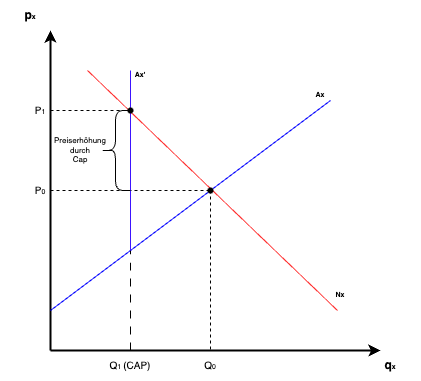
\includegraphics[width=0.8\textwidth]{Bilder/supply_demand_ets.png} 
	\caption{Angebot und Nachfrage von Emissionszertifikaten mit CAP (vgl. \cite{pettinger.2017})}
	\label{fig:supply_demand_ets}
\end{figure}